\documentclass[10pt,aspectratio=169,mathserif]{beamer}

%%%%-----导入宏包-----%%%%
\usepackage{seu}
\usepackage{xeCJK}
\usepackage{amsmath,amsfonts,amssymb,bm}
\usepackage{color}
\usepackage{graphicx,hyperref,url}
\usepackage{booktabs}
\usepackage{tikz}
\usetikzlibrary{positioning,arrows.meta,calc}
%%%%%%%%%%%%%%%%%%

%%%%-----设置字体-----%%%%
\setsansfont[Path=fonts/]{Helvetica}
\setCJKmainfont[Path=C:/Windows/Fonts/,BoldFont=simhei.ttf,ItalicFont=simkai.ttf]{simsun.ttc}
\setCJKsansfont[Path=C:/Windows/Fonts/,BoldFont=msyhbd.ttc,AutoFakeBold=2]{msyh.ttc}
\setCJKmonofont[Path=C:/Windows/Fonts/]{simfang.ttf}

\definecolor{comp}{RGB}{46,110,158}
\definecolor{rout}{RGB}{192,80,77}
\definecolor{both}{RGB}{107,78,155}
\definecolor{seugreen}{RGB}{81,122,52}

\beamertemplateballitem

% 片子只有 13 页，不为每个 section 插播目录页（否则页数翻倍）
% \AtBeginSection[] { ... \tableofcontents[currentsection] ... }

%%%%----首页信息设置----%%%%
\title[压缩与路由]{压缩与路由：自注意力快权重的两个缩放算子}
\subtitle{\fontsize{9pt}{14pt}\selectfont \textbf{Compression--Routing Correspondence —— 一次可证伪的统一验证}}
\author[汪涵]{
  汪涵 \\\medskip
  {\small 指导教师：待补}}
\institute[SEU]{东南大学\quad 集成电路学院}
\date[2026.11]{2026 年 11 月}

\begin{document}

%%%% ============ 封面 ============
\begin{frame}
\titlepage
\end{frame}

%%%% ============ 目录 ============
\section*{目录}
\begin{frame}
\frametitle{\textbf{目录}}
\textbf{\tableofcontents}
\end{frame}

%%%% ============ 1 问题 ============
\section[问题]{问题：两族方法，缺一个共同坐标}

\begin{frame}
\frametitle{\textbf{两族高效注意力，各自有一套故事}}
  \begin{columns}[T]
    \column{.48\textwidth}
      \begin{block}{\textbf{压缩族}}
        \footnotesize
        Linformer、Performer、Nystr\"om、块池化 \\
        \medskip
        做法：用一组全局共享的槽位概括全部 key \\
        \medskip
        几何含义：$W$ 被压成\textbf{低秩}
      \end{block}

    \column{.48\textwidth}
      \begin{block}{\textbf{路由族}}
        \footnotesize
        Top-$k$ attention、MoBA、Agent、稀疏注意力 \\
        \medskip
        做法：每个 query 只挑选少量 key 参与 \\
        \medskip
        几何含义：$W$ \textbf{满秩但每行稀疏}
      \end{block}
  \end{columns}

  \vspace{0.5em}
  \begin{block}{\textbf{缺的那句话}}
    \small
    两族都能解释自己为什么省算力，但很少回答：\textbf{它们是不是同一个对象上的两种操作？}
    如果是，那么这个操作在对象上应当有唯一的最优形式，而不是一堆互不相干的工程技巧。
  \end{block}
\end{frame}

%%%% ============ 2 形式化 ============
\section[形式化]{统一形式化：一个对象，两个约束}

\begin{frame}
\frametitle{\textbf{把注意力看成动态快权重 MLP}}
  \begin{center}
    \large
    $y = W(x)\,V$，\qquad $W(x)=\mathrm{softmax}\!\left(QK^{\top}/\sqrt{d}\right)\in\mathbb{R}^{N\times N}$
  \end{center}

  \vspace{0.3em}
  \begin{center}
  \begin{tikzpicture}[x=0.95cm,y=0.95cm,font=\scriptsize]
    % (1) 稠密 W
    \fill[gray!18] (0,0) rectangle (1.68,1.68);
    \draw[step=0.42,gray!55] (0,0) grid (1.68,1.68);
    \node[below=3pt] at (0.84,0) {稠密 $W(x)$};
    % (2) 压缩后：所有行落在同一子空间（示意为各行相同）
    \begin{scope}[xshift=4.2cm]
      \draw[step=0.42,gray!55] (0,0) grid (1.68,1.68);
      \foreach \j in {0,1,2,3} {%
        \fill[comp!55] (0.00,\j*0.42) rectangle ++(0.42,0.42);
        \fill[comp!55] (0.84,\j*0.42) rectangle ++(0.42,0.42);}
      \node[below=3pt] at (0.84,0) {压缩：$\mathrm{rank}\,W\le r$};
    \end{scope}
    % (3) 路由后：每行只留 k 个
    \begin{scope}[xshift=8.4cm]
      \draw[step=0.42,gray!55] (0,0) grid (1.68,1.68);
      \foreach \j in {0,1,2,3} {%
        \fill[rout!70] (\j*0.42,\j*0.42) rectangle ++(0.42,0.42);}
      \node[below=3pt] at (0.84,0) {路由：$\mathrm{nnz}$/行 $\le k$};
    \end{scope}
  \end{tikzpicture}
  \end{center}

  \vspace{0.2em}
  \begin{columns}[T]
    \column{.5\textwidth}
      \footnotesize
      \textcolor{comp}{\textbf{压缩}}：$W\to AE$，$E$ 全局共享
      $\Rightarrow$ 投影到“秩 $\le r$”的集合\\
      最优近似 = 截断 SVD（Eckart--Young）
    \column{.5\textwidth}
      \footnotesize
      \textcolor{rout}{\textbf{路由}}：$W\to W\odot M_k$，逐行留 $k$ 个
      $\Rightarrow$ 投影到“每行 $\le k$”的集合\\
      最优近似 = 逐行取绝对值最大的 $k$ 个
  \end{columns}
\end{frame}

%%%% ============ 3 MiTA ============
\begin{frame}
\frametitle{\textbf{MiTA：两项相加，恰好落在两轴的并集上}}
  \begin{center}
    $W \;=\; \underbrace{\alpha\,S}_{\text{压缩项}} \;+\; \underbrace{\beta}_{\text{路由项}}$,
    \qquad
    $y=\sum_{m}\alpha_m\!\left(\sum_j S_{mj}v_j\right)+\sum_j \beta_j v_j$
  \end{center}

  \begin{itemize}
    \small
    \item $S$：$M$ 个与 query 无关的\textbf{压缩专家}槽位（router 用池化网格生成）$\Rightarrow$ 低秩
    \item $\beta$：被选中的专家所携带的 top-$k$ KV（MoBA 段）$\Rightarrow$ 行稀疏
    \item 两项在\textbf{同一次联合 softmax} 中相加 —— 这正是官方实现把 agent 段与 MoBA 段
          拼进一个 varlen 调用的几何含义
  \end{itemize}

  \vspace{0.4em}
  \begin{block}{\textbf{一个直接推论}}
    \small
    $W=\alpha S+\beta$ 既不是低秩的，也不是稀疏的。
    所以只用“低秩”或只用“稀疏”去描述它都会\textbf{漏掉一半}；
    只有在“两轴共同张成的空间”里，它才是一个自然对象。
  \end{block}
\end{frame}

%%%% ============ 4 断言 ============
\section[断言]{三条可证伪的断言}

\begin{frame}
\frametitle{\textbf{把命题拆成三条可证伪的断言}}
  \begin{center}
  \footnotesize
  \begin{tabular}{@{}p{2.4cm}p{6.9cm}p{3.7cm}@{}}
    \toprule
    \textbf{断言} & \textbf{内容} & \textbf{由谁验证} \\
    \midrule
    \textcolor{seugreen}{\textbf{A1 对应性}} &
    压缩 $\equiv$ 投影到 $\{\text{rank}\le r\}$；路由 $\equiv$ 投影到 $\{\mathrm{nnz}/\text{行}\le k\}$，
    且两者都是\textbf{最优闭式解} &
    E1（解析，无需训练） \\
    \addlinespace
    \textcolor{seugreen}{\textbf{A2 正交性}} &
    两个旋钮各自只推动自己的统计量与成本，\textbf{互不替代} &
    E2（短训 + 结构量） \\
    \addlinespace
    \textcolor{seugreen}{\textbf{A3 可叠加性}} &
    真实训练下两种约束\textbf{可共存}，缺的一项可低成本补插 &
    E3（CIFAR-100 2$\times$2） \\
    \bottomrule
  \end{tabular}
  \end{center}

  \vspace{0.6em}
  \begin{columns}[T]
    \column{.5\textwidth}
      \footnotesize
      \textbf{两个结构量}（都从导出的精确 $W$ 上测，不用代理指标）\\[2pt]
      $\rho=\mathrm{stable\_rank}(W)/N$ \quad 横轴：压缩 \\
      $\mathrm{pr}=$ 每 query 有效 keys 数 $/N$ \quad 纵轴：路由
    \column{.5\textwidth}
      \footnotesize
      \textbf{一句免责}：本工作验证的是\textbf{结构对应关系}，\\
      不宣称任何 SOTA 精度，也不与 ImageNet 数字对齐。
  \end{columns}
\end{frame}

%%%% ============ E1 方法 ============
\section[E1]{E1 · 两个约束的闭式投影}

\begin{frame}
\frametitle{\textbf{E1：为什么这个实验不需要训练}}
  \begin{block}{\textbf{关键事实}}
    \small
    两个约束集上的\textbf{最优}近似都有闭式解，所以只要构造结构已知的 $W^{*}$，
    量它到两个约束集的距离，就能得到解析边界 —— 不需要任何梯度。
  \end{block}

  \vspace{0.2em}
  \begin{center}
  \footnotesize
  \begin{tabular}{@{}p{1.9cm}p{4.4cm}p{4.0cm}p{4.0cm}@{}}
    \toprule
    \textbf{探针} & \textbf{$W^{*}$} & \textbf{秩投影何时精确} & \textbf{支撑投影何时精确} \\
    \midrule
    P1 & 低秩稠密 $uv^{\top}$，秩 1 & $r=1$ & $k\to N$ \\
    P2 & 满秩稀疏，置换阵 & $r\to N$（永不提前） & $k=1$ \\
    P3 & 满秩稠密，高斯 & $r=N$ & $k=N$ \\
    P4 & 低秩 + 稀疏，两者各半 & 预算饱和才达标 & 预算饱和才达标 \\
    \bottomrule
  \end{tabular}
  \end{center}

  \vspace{0.3em}
  \footnotesize
  $\Rightarrow$ 这是一个\textbf{交叉模式}：P2 的两种投影在预算很小的时候就分道扬镳。
  若两族真是同一个操作，P2 的两条曲线必须重合 —— 它们没有。
\end{frame}

%%%% ============ E1 结果 ============
\begin{frame}
\frametitle{\textbf{E1 结果：路由的不可替代性有了硬证据}}
  \begin{center}
    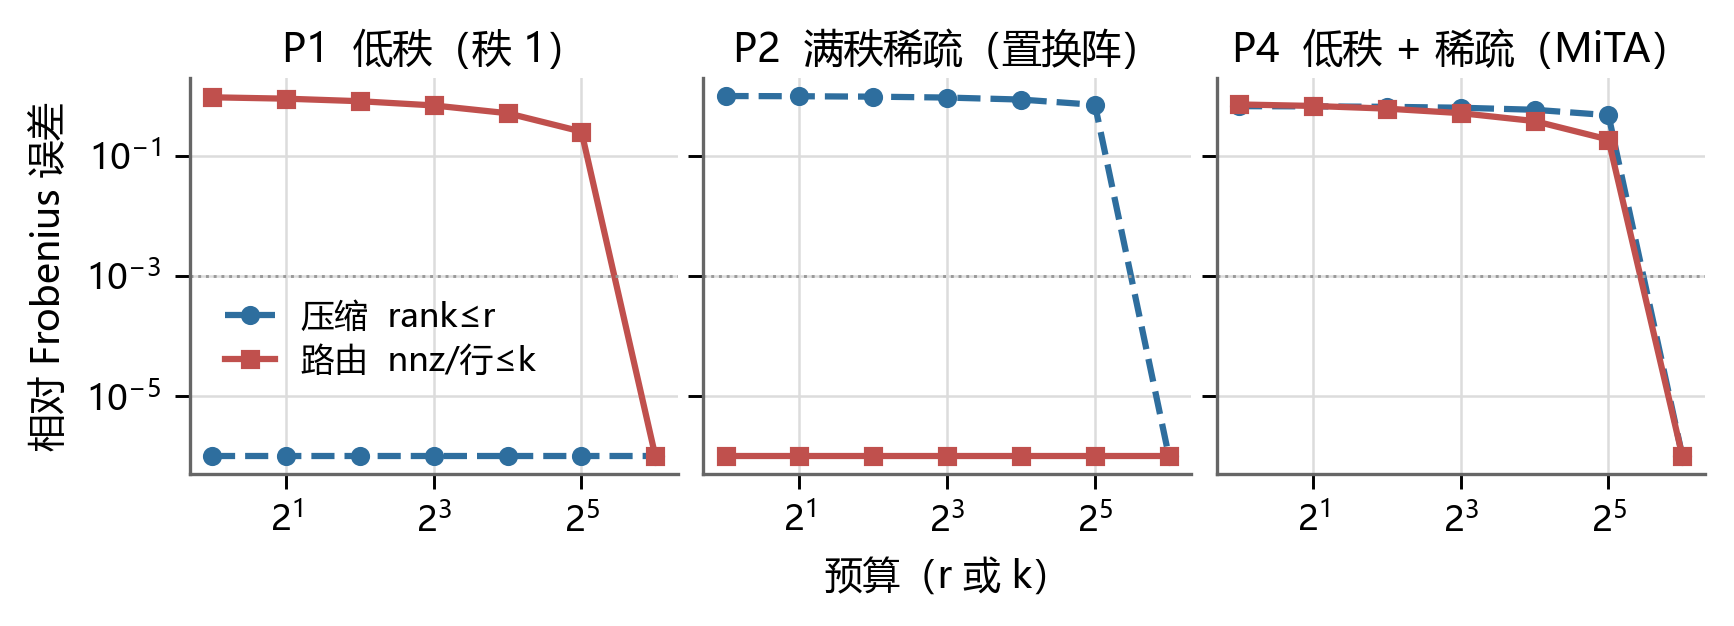
\includegraphics[width=\textwidth]{figures/fig_e1.png}
  \end{center}

  \vspace{-0.4em}
  \begin{columns}[T]
    \column{.48\textwidth}
      \footnotesize
      \textbf{P2（置换阵）}：$r=32$ 即半个预算，秩投影误差仍是 $\mathbf{0.707}$；
      一路到 $r=64$ 才归零。同一矩阵的支撑投影 $k=1$ 就已经精确为 $0$。
    \column{.48\textwidth}
      \footnotesize
      \textbf{P4（MiTA 形状）}：两条曲线在预算饱和前都下不去 ——
      残余需要\textbf{两项一起}才能消掉。这就是“并集”的形状学证据。
  \end{columns}
\end{frame}

%%%% ============ E2 ============
\section[E2]{E2 · 两个旋钮各推各的统计量}

\begin{frame}
\frametitle{\textbf{E2：支撑约束\textbf{写在} $W$ 里，秩约束只是一个容量上界}}
  \begin{center}
    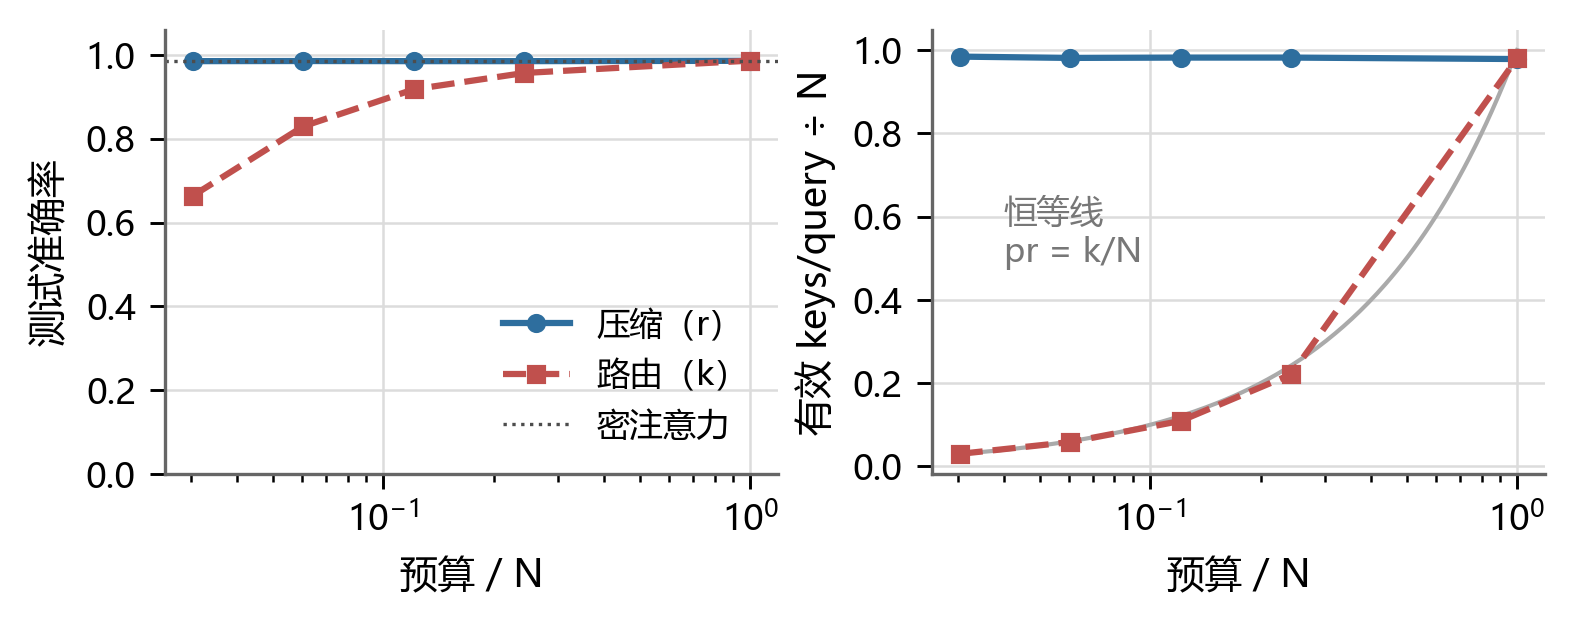
\includegraphics[width=0.93\textwidth]{figures/fig_e2.png}
  \end{center}

  \vspace{-0.6em}
  \begin{columns}[T]
    \column{.5\textwidth}
      \footnotesize
      \textbf{任务}：多数投票 —— 标签取决于两候选值在整条序列中的计数，
      所以必须真的看到足够多的 key，路由预算才会疼。\\[3pt]
      \textcolor{rout}{$\mathrm{pr}$ 逐点等于 $k/N$}（$k=1$ 精确到 $1/33$）
      $\Rightarrow$ 路由就是把 $W$ 的支撑截断
    \column{.5\textwidth}
      \footnotesize
      \textbf{成本不对称}：$k$ 压到 1，准确率 $0.986\to0.664$；
      $r$ 压到 1，几乎不动（$0.9852$）。\\[3pt]
      \textcolor{seugreen}{\textbf{负面结果}}：$\rho$ 恒在 $0.03$，不随 $r$ 变。
      秩约束是\textbf{容量陈述}，不是可观测统计量 —— 这正是 E1 存在的理由。
  \end{columns}
\end{frame}

%%%% ============ E3 设计 ============
\section[E3]{E3 · 真实训练下的可叠加性}

\begin{frame}
\frametitle{\textbf{E3：2$\times$2 因子设计 + 阴性对照}}
  \begin{center}
  \footnotesize
  \begin{tabular}{@{}lcccl@{}}
    \toprule
    \textbf{变体} & \textbf{压缩} & \textbf{路由} & \textbf{对应方法} & \textbf{作用} \\
    \midrule
    \texttt{dense} & $\times$ & $\times$ & 标准注意力 & 基线 \\
    \texttt{linformer} $r{=}64$ & \checkmark & $\times$ & Linformer / Performer & 只有压缩 \\
    \texttt{topk} $k{=}64$ & $\times$ & \checkmark & MoBA / top-$k$ & 只有路由 \\
    \texttt{mita} $r{=}k{=}64$ & \checkmark & \checkmark & MiTA & 两项并存 \\
    \midrule
    \texttt{dense\_dwc} / \texttt{dense\_gate} & — & — & DWC、SiLU 门控 & \textbf{阴性对照} \\
    \bottomrule
  \end{tabular}
  \end{center}

  \vspace{0.3em}
  \begin{columns}[T]
    \column{.52\textwidth}
      \footnotesize
      \textbf{阴性对照是这套设计不被判“什么都能解释”的关键}：\\
      DWC 与门控确实涨点，但它们\textbf{不沿任何一条轴}移动。
      若对照点也动了，两轴故事当场被证伪。
    \column{.44\textwidth}
      \footnotesize
      \textbf{iso-FLOPs 记账口径}：\\
      \textcolor{comp}{压缩}：省 $K^{\top}V$ 与 $AV$ 两块\\
      \textcolor{rout}{路由}：只省 $AV$（打分仍需 $q\cdot k$）
  \end{columns}
\end{frame}

%%%% ============ E3 结果 ============
\begin{frame}
\frametitle{\textbf{E3 结果：交互项为正，且比两个主效应都大}}
  \begin{center}
    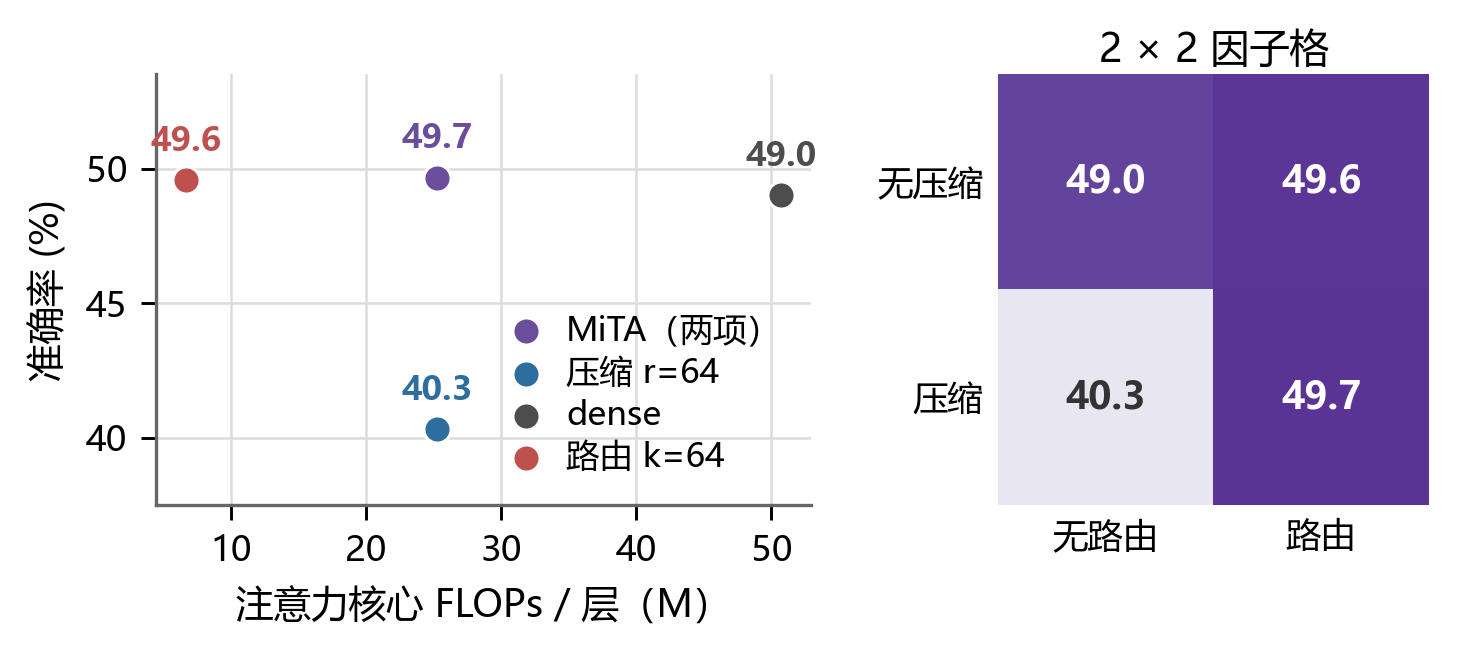
\includegraphics[width=0.78\textwidth]{figures/fig_e3.png}
  \end{center}

  \vspace{-0.5em}
  \begin{columns}[T]
    \column{.56\textwidth}
      \scriptsize
      口径：CIFAR-100，128 px / patch 8 $\Rightarrow N=257$，$r=k=64$（预算 25\%），
      20 epoch，单种子，单卡 3060。\\[4pt]
      主效应：\textcolor{comp}{压缩 $-4.31$ pt}，\textcolor{rout}{路由 $+4.95$ pt}，
      交互 \textbf{$+8.80$ pt} —— 压缩单独掉 8.7 pt，并集没有继承这个损失。
    \column{.42\textwidth}
      \footnotesize
      \textbf{能说}：压缩破坏了可路由性，并集把它救了回来。\\[4pt]
      \textbf{不能说}：MiTA 比 dense 高 0.64 pt —— 单种子、20 epoch，落在噪声内，
      只能说“没有损失”。
  \end{columns}
\end{frame}

%%%% ============ 结论 ============
\section[结论]{结论与边界}

\begin{frame}
\frametitle{\textbf{结论：一个对象，两个正交的缩放算子}}
  \begin{block}{\textbf{站得住的三条}}
    \small
    \begin{enumerate}
      \item \textbf{A1 对应性}：压缩与路由分别是 $W$ 到两个约束集的\textbf{最优}投影，
            且最优解都是闭式的（SVD / 行 top-$k$）—— E1 给出解析边界。
      \item \textbf{A2 正交性}：路由把支撑精确写进 $W$（$\mathrm{pr}=k/N$ 逐点吻合），
            压缩把 $W$ 抹平（$\mathrm{pr}\to0.98$），二者互不替代 —— E2。
      \item \textbf{A3 可叠加性}：真实训练里两者共存，且交互项 $+8.80$ pt —— E3。
    \end{enumerate}
  \end{block}

  \begin{columns}[T]
    \column{.5\textwidth}
      \begin{block}{\textbf{要说清楚的边界}}
        \footnotesize
        $\rho$ 作为横轴\textbf{不可观测}（E1 之所以必需）；\\
        \texttt{topk} 的 6.7 M 是\textbf{算法渐近}成本，
        参考实现为导出精确 $W$ 反而更慢；\\
        微型模型 + 单种子，结论是结构性的。
      \end{block}
    \column{.46\textwidth}
      \begin{block}{\textbf{下一步}}
        \footnotesize
        把两轴统计量做到 patch 级与 head 级（而非整层）；\\
        在 DeiT-T 配置上复核交互项；\\
        用本套件做新注意力算子的\textbf{归类测试}。
      \end{block}
  \end{columns}
\end{frame}

%%%% ============ 致谢 ============
\section*{}
\begin{frame}
  \begin{center}
    \begin{minipage}{1\textwidth}
      \setbeamercolor{mybox}{fg=white, bg=black!60!seugreen}
      \begin{beamercolorbox}[wd=0.70\textwidth, rounded=true, shadow=true]{mybox}
      \LARGE \centering Thanks for Listening.
      \end{beamercolorbox}
    \end{minipage}
  \end{center}

  \vspace{0.6em}
  \begin{center}
    \small
    实验代码：\texttt{experiments/}（E1 解析 · E2 旋钮扫描 · E3 iso-FLOPs 四格）\\
    全部为\textbf{从零实现}的参考实现，不依赖 flash-attn，CPU 可复现
  \end{center}
\end{frame}

\end{document}
